\newcommand{\wallH}{0.6} % = wall height
\newcommand{\lineW}{6} % = line width
\newcommand{\lineH}{0.8} % = line height diff
\newcommand{\size}{2.3} % Tjocklek på linjerna

\newcommand{\arrow}{1.5} % Tjocklek på pilarna

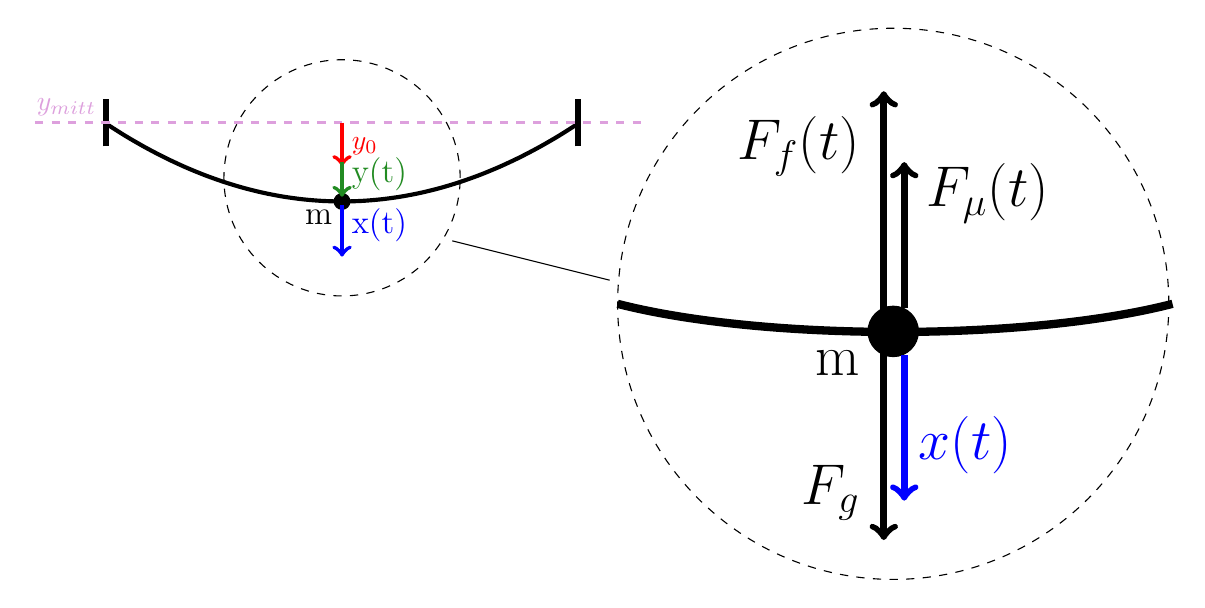
\begin{tikzpicture}

% Två raka sträck som håller i linan
\draw [line width=\size] (0,0) -- (0,\wallH);
\draw [line width=\size] (\lineW,0) -- (\lineW,\wallH);


% Själva linan
%\draw [line width=1.5] (0,\wallH/2)  arc[x radius=\lineW/2, y radius=\lineH, start angle=180, end angle=360];
%\draw [line width=1.5] (0,\wallH/2) arc (180:360:\lineW/2 and \lineH);
\draw [line width=1.5, domain=0:\lineW, smooth, variable=\x] plot ({\x},{-0.7+ 0.11*(\x-\lineW/2)*(\x-\lineW/2)});

% Mittlinje
\draw [line width=1.2, dashed, Plum] (-0.9,0.3) -- (\lineW+0.9,0.3);
\node [left, Plum] at (0, 0.5) {$y_{mitt}$};

% punkt m
\draw [fill] (\lineW/2, -0.7) circle [radius=0.1];
\node [left] at (\lineW/2, -0.9) {\large m};

% y_0
\draw [->, line width=\arrow, red] (\lineW/2, 0.3) -- (\lineW/2,-0.25);
\node [right, red] at (\lineW/2, 0) {$y_{0}$};

% y(t)
\draw [->, line width=\arrow, ForestGreen] (\lineW/2, -0.2) -- (\lineW/2, -0.64);
\node [right, ForestGreen] at (\lineW/2, -0.35) {\large y(t)};

% x(t)
\draw [->, line width=\arrow, Blue] (\lineW/2, -0.75) -- (\lineW/2, -1.4);
\node [right, Blue] at (\lineW/2, -1) {\large x(t)};

% d
%\node [centered] at (1.5, -1.1) {\large d};
%\draw [<->, line width=1] (0, -0.8) -- (3, -0.8);

% liten zoom-cirkel
\draw [dashed] (\lineW/2, -0.4) circle [radius=1.5];

% stor zoom-cirkel
\draw [dashed] (\lineW + 4, -2) circle [radius=3.5];

% linje mellan cirklarna
\draw (4.4, -1.2) -- (6.4,-1.7);

% stor lina
\draw [line width=3]  (6.5,-2) arc (220:320:4.6 and 1);

% stor Refenslinje
%\draw [line width=1.2, dashed, red] (7.1,-3.9) -- (12.95,-3.9);

% stor Mittlinje
%\draw [line width=1.2, dashed, Plum] (6.6,-1.1) -- (13.4,-1.1);

% stor punkt
\draw [fill] (10, -2.35) circle [radius=0.32];

% stort m
\node [left] at (9.7, -2.75) {\huge m};

% kraft: f
\draw [->, line width=2.5] (9.88, -2.35) -- (9.88, 0.7);
\node [left] at (9.7, 0) {\huge $F_{f}(t)$};

% kraft: g
\draw [->, line width=2.5] (9.88, -2.35) -- (9.88, -5);
\node [left] at (9.7, -4.4) {\huge $F_g$};

% stor x(t)
\draw [->, line width=2.5, Blue] (10.14, -2.65) -- (10.14, -4.5);
\node [right, Blue] at (10.2, -3.8) {\huge $x(t)$};

% kraft: my
\draw [<-, line width=2.5] (10.14, -0.2) -- (10.14, -2.05);
\node [right] at (10.3, -0.6) {\huge $F_{\mu}(t)$};

% Fs1
%\draw [->, line width=2.5] (9.88, -2.35) -- (6.88, -0.8);
%\node [right] at (6.6, -1.7) {\Large $F_{s1}(t)$};

% Fs2
%\draw [->, line width=2.5] (10.14, -2.35) -- (13.22, -0.8);
%\node [left] at (13.4, -1.7) {\Large $F_{s2}(t)$};

\end{tikzpicture}